%\documentclass[linenumbers, RNAAS, trackchanges]{aastex631}
\documentclass{aastex631}
%\documentclass[manuscript]{aastex631}
%\documentclass[a4paper, 10pt]{article}

\usepackage[utf8]{inputenc}
\usepackage{hyperref}           % hrefs
\usepackage{natbib}             % for bibliography
\usepackage{float}              % figure positioning
\usepackage{svg}                % used for SVG images
\usepackage{graphicx}           % used for non-SVG images
\usepackage{amsmath}

% Search Query Metadata
\shorttitle{Logistic Map}
\shortauthors{Corresponding Author's Last Name, et al.}

% Hyperlink setup
\hypersetup{
colorlinks=true,
linkcolor=blue,
urlcolor=blue
}

\begin{document}
\title{Bifurcation and Chaos in the Logistic Map}
% [] is for ORCiD
%\correspondingauthor{Main Author}
%\email{author1@email.com, author2@email.com, author3@email.com}
\author{Lily Nguyen}
\affiliation{Department of Physics, The University of Texas at Austin\\
Austin, TX 78712, USA}

\author{Raymond Vu}
\affiliation{Department of ---, The University of Texas at Austin\\
Austin, TX 78712, USA}

%\thanks{These authors contributed equally to this work.}

%\collaboration{2}{CS 323E}
% or 
%\nocollaboration{0}

% 250 word limit for abstract
\begin{abstract}
This is the abstract. The word limit is 250.


\end{abstract}

% Use astrothesaurus numbers in place of num
\keywords{keyword 1 (num) --- keyword 2 (num) --- keyword 3 (num)}
\section{Introduction} \label{sec:intro}
This is the intro section.

\section{Data} \label{sec:data}
This is the data section.

Maybe add some lists/tables/whatever is needed.



\section{Information about Observations}
Write info about observations here.

\subsection{Specific Topic Pt 1} \label{sec:subtopic1}
topic 1

\subsection{Specific Topic Pt 2} \label{sec:subtopic2}
topic 2

\begin{figure}[H]
    \centering
    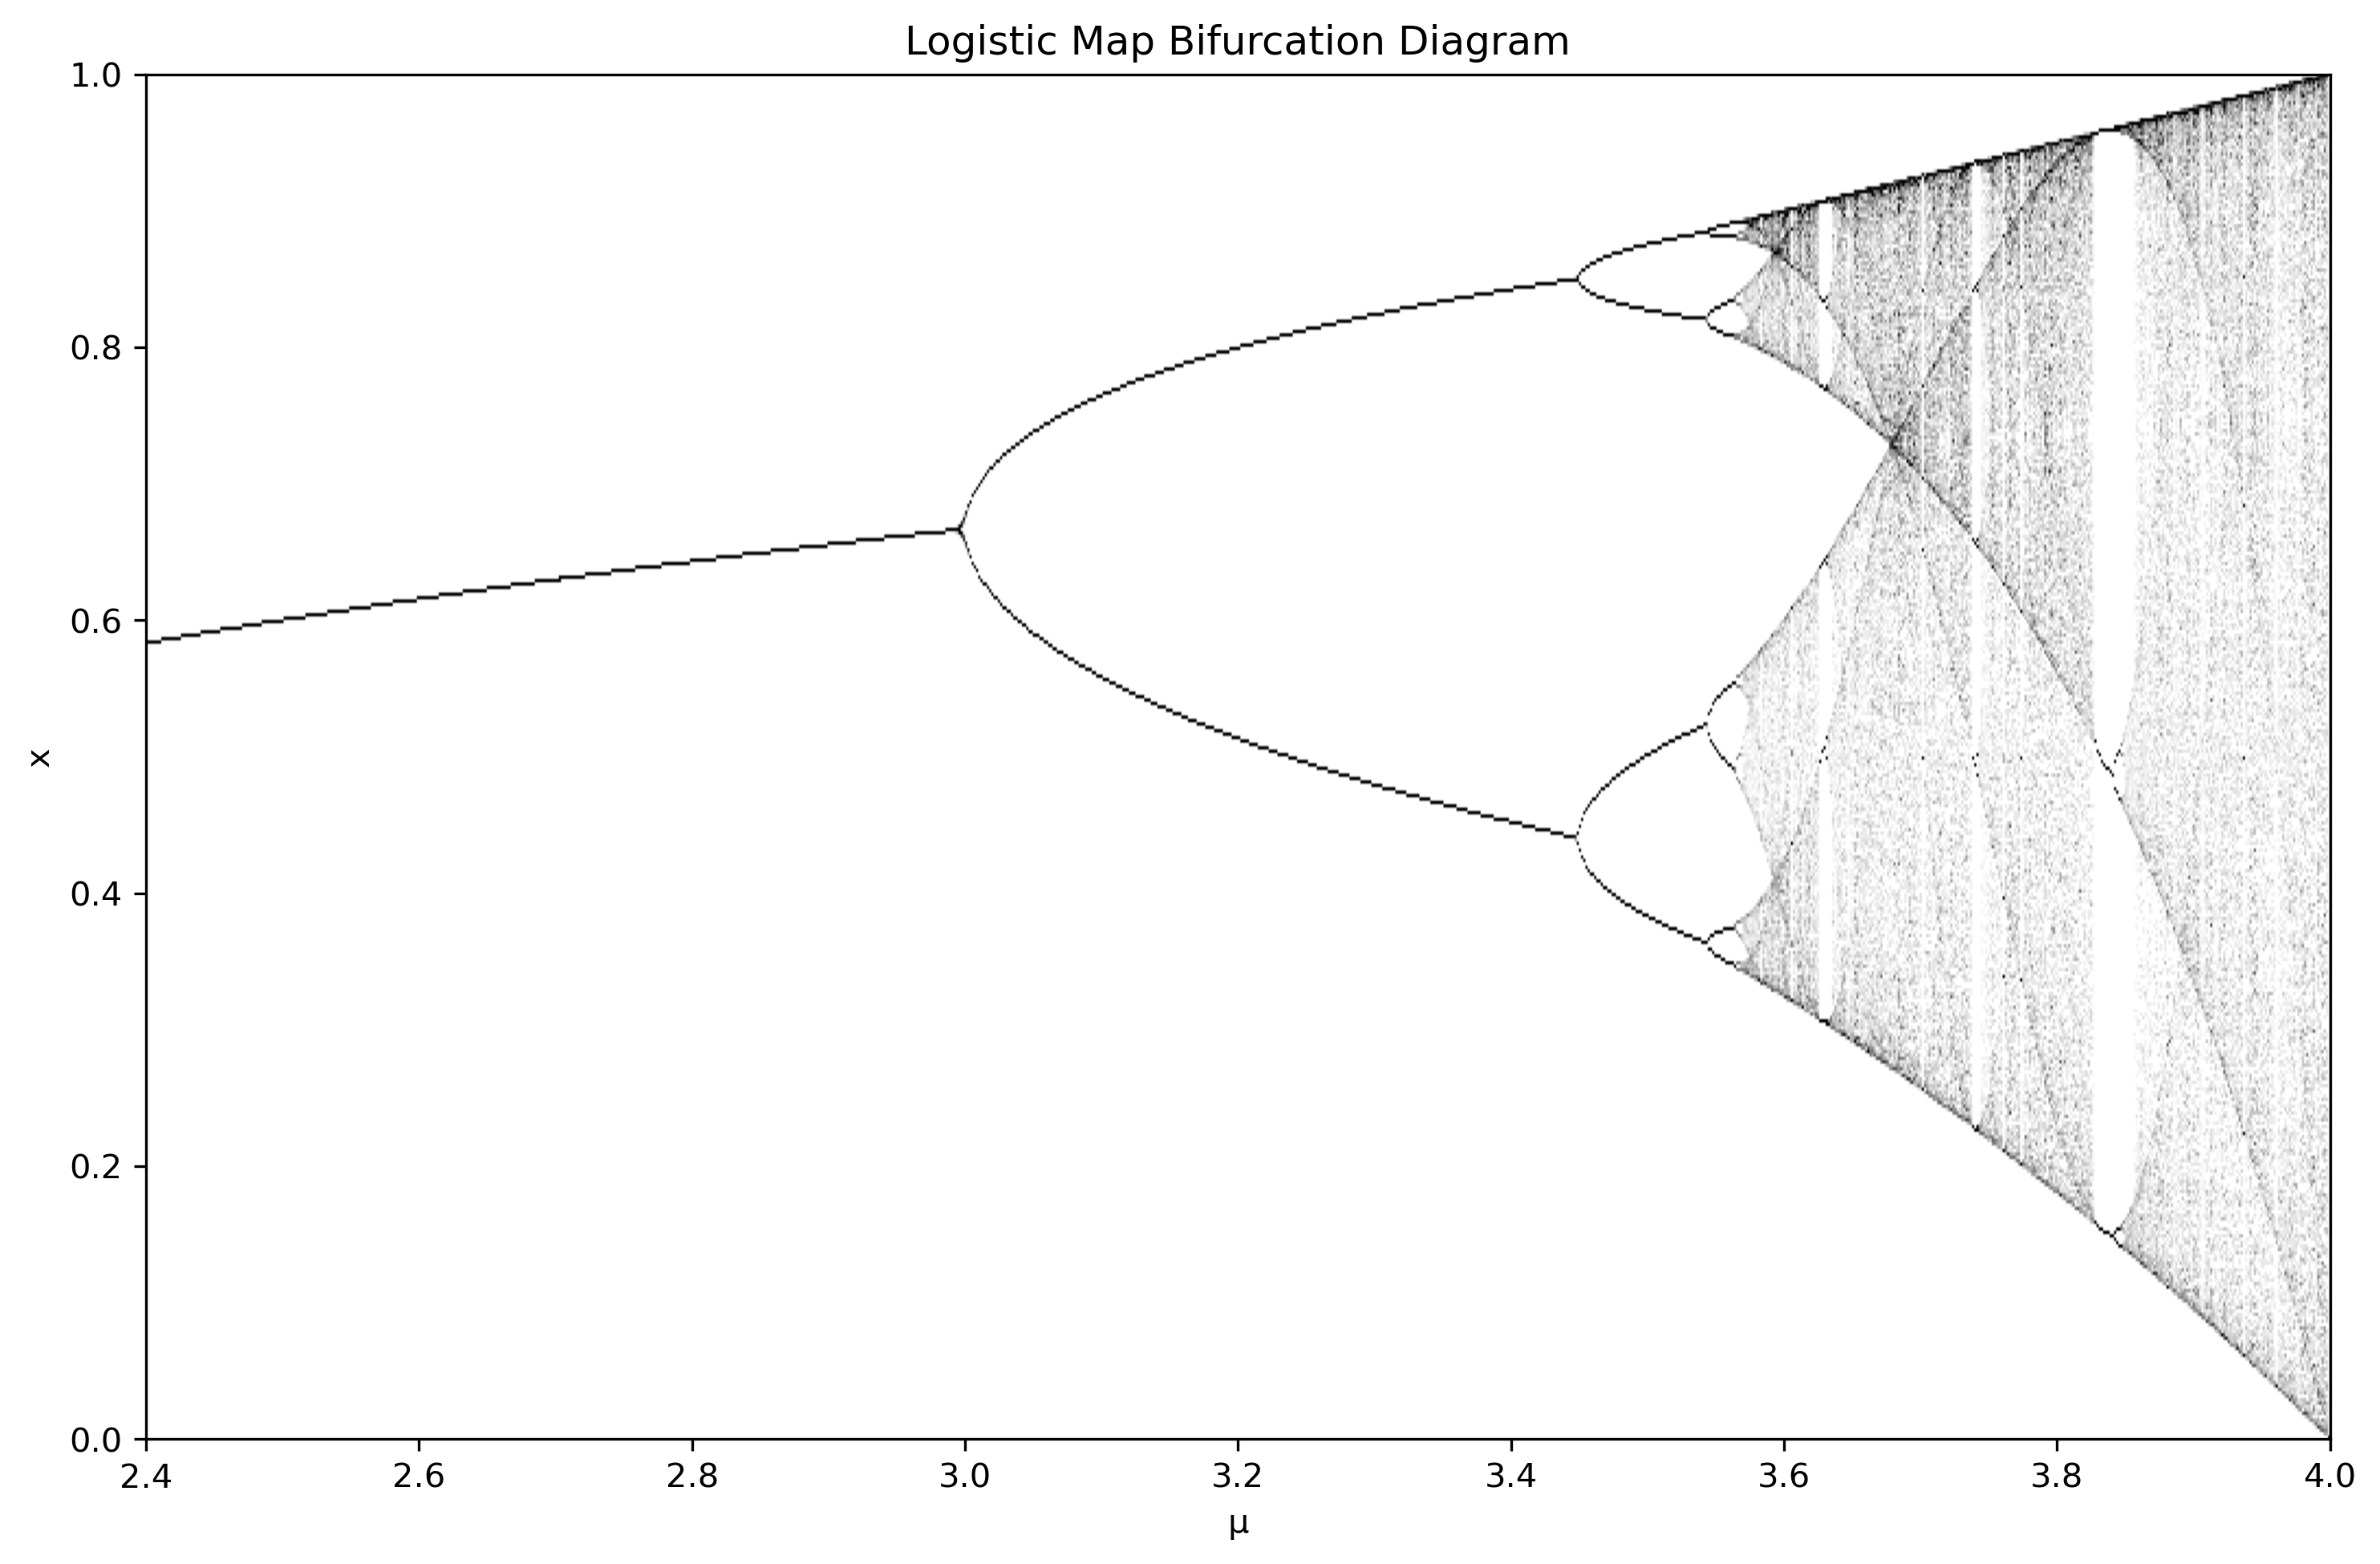
\includegraphics[width=0.9\linewidth]{bifurcation.png}
    \caption{The logistic map bifurcation diagram for $2.4\leq \mu \leq 4.0$. Stable fixed points exist for low values of $\mu$, followed by successive period-doubling bifurcations that lead to chaotic behavior near $\mu\approx 3.57$.}
    \label{fig:bifurcation}
\end{figure}


\subsection{Specific Topic Pt 3} \label{sec:subtopic3}
topic 3

\section{Results} \label{sec:results}
write about the results here.


\section{Summary and Conclusion} \label{sec:summary}
Put the summary and conclusions here.


\subsubsection{References}
This is me citing \citet{boeing} in-text. This is me citing Bubolo at the end of this sentence \citep{bubolo}.

\newpage
\bibliographystyle{aasjournal}
%\bibliographystyle{plainnat}
\bibliography{refs}

\end{document}
